\setlength{\parindent}{0em}
\setlength{\parskip}{1em}
\chapter{Introduction}

Linux distributions are build upon packages which provide software to their users. It is these
packages that make particular distribution different or similar to other one. All these packages require
maintenance, in the case the distribution is developed commercially, as well as it is developed by community.
The fact that the whole system is stable and comfortable to use is a result of a good work of
maintainers who work together to ensure that all packages are working and their
requirements are met.

An efficient maintenance requires accurate information which maintainers get from multiple sources
and are using many tools to retrieve. For example, which packages depend on their own packages and thus which
maintainers should they communicate with when encountering disturbing changes. Often the information
is not easy to acquire and slows down developers by forcing them to manually search through different
places. To solve this problem a new tool which is able to store and filter any information about
packages is required as no other exist in the moment of making this thesis.

RPQR is an originally proposed tool which is supposed to make maintainers life easier by allowing them to describe how
to acquire the data only once and then being able to retrieve it on demand. It is flexible
enough to store any new kind of data and to search packages based on combination of any of them while
also providing the option to accelerate queries by making specialized commands.
RPQR also lets users build a cache which makes further queries faster and thus saves time while
doing everyday work.

the tool is able to be directly used by other projects through provided API or it can be used
by user as any other command line project. Users are also able to visualize their
results for faster understanding of the results.

\chapter{Theory and current state}
While crucial information about a RPM package is stored directly inside it within the header section,
additional information as who maintains it or which bugs are currently known has to be searched
in external sources of information. This chapter describes RPM packages and technologies which
currently exist for working with them. Then we continue with a description of other subjects which are needed
to successfully design and implement RPQR project.

\section{RPM package}
RPM packages have their own file format\cite{RPMFileFormat}. It is composed of four parts with their specific purposes.
The parts are (i)lead, (ii)signature, (iii)header and (iv)archive. Here are described and explained all parts
relevant to the RPQR project.

\subsection*{The lead}
The lead is the first part of the RPM package. It contains magic number and version of RPM file format.
It also contains whether the package type is binary or source and other information relevant
for system using it. The difference between binary and source package is that source package contains
source code from which software can be built or the whole downloaded project, while binary package
contains the actual software. The lead is no longer used internally by RPM because of its
inflexibility and is noted here only for completeness of file format description.

\subsection*{The signature}
The signature is allowing package integrity and optionally authenticity to be verified. It holds
little purpose for RPQR but it is important because dnf uses it and RPQR is using dnf API.

\subsection*{The header}
The header is the most interesting part from perspective of RPQR project, because it contains
detailed crucial information about the package. It is composed of tags which describe different
aspects of the bundled software. Examples of these tags can be \mbox{\textit{RPMTAG\_VERSION}}
specifying version of the package or \textit{RPMTAG\_RELEASE} which specifies what release of
this version this is. Header is parsed by a software which is making metadata structure of RPM
repositories and this structure is then used by the dnf package manager to find appropriate
packages that the user needs.

\begin{lstlisting}
00001198  8e ad e8 01 00 00 00 00  00 00 00 3e 00 00 0f dd  |...........>....|
\end{lstlisting}

The first 16 bytes of header part are describing attributes of this header. Three bytes are
magic number identifying header, one byte says that header conforms to version 1 of specification.
Four another bytes are reserved and then there is count of entries stored in this header
(00 00 00 3e to decimal is 62). The last four bytes mean how many bytes is stored in this structure
(00 00 0f dd to decimal is 4061).

\begin{lstlisting}
000011c8  00 00 03 e8 00 00 00 06  00 00 00 02 00 00 00 01  |................|
\end{lstlisting}

For best example, we will describe name tag. 00 00 03 e8 identifies presence of
name tag and 00 00 00 06 says that value is string. 00 00 00 02 means that value
is located 2 bytes after the start of store and 00 00 00 01 indicates that there is
just one value, which is the only allowed possibility for string value stored in the header.

The store is just values after each other and are distinguished only by their respective offsets.

\subsection*{The archive}
The archive is a set of files and folders compressed with a compression algorithm. Its integrity
can be verified with signature specified.

\section{RPM repository}
RPM repositories are directory structures which contain RPM packages and metadata which are needed
to quickly locate packages that user needs. Metadata are created by createrepo \cite{RPMRepository}
utility and accessed by dnf package manager. 

\subsection*{Repodata}
Every RPM repository contains folder \textit{repodata} which contains data about contents of the
repository. There is a file \textit{repomd.xml} containing xml structure indicating where should
package manager look for databases with information about packages.

Important databases:
\begin{itemize}
  \item \textbf{primary} database which specifies all crucial information about each package as version, description or file list.
  \item \textbf{other} database which contains other less important information e.g. changelog of a package
\end{itemize}

\section{Package managers}
Work with RPM packages can be done by multiple tools. Their general responsibility is to recognize
package dependencies and being able to install or uninstall software contained in the package.
Most frequently used are RPM package manager and DNF package manager (successor of the old
YUM package manager).

\subsection*{RPM package manager}
RPM package manager supports more low level operations with packages than DNF does \cite{RPMPackageManager}. It allows
to build source of a project according to specfile and create distributable packages. More of the
important operations are also reading of the metadata and verification of installed software, in
case that it is not working properly. Installation of dependencies would have to be handled by user
manually so rpm utility is not often used by end users of the systems.

\subsection*{YUM package manager}
Yum package manager is historically the first manager that allowed easy downloading of packages
from remote repositories and handling their dependencies \cite{YUMPackageManager}. It is currently deprecated and has been
replaced by DNF. Reasons for deprecation and replacement were that YUM was not properly documented,
it was not ready for switch to python3 and algorithm for dependency resolvement was not strong enough
to handle all problems that withstand in modern RPM based linux distributions.

\subsection*{DNF package manager}
DNF package manager is a successor of the older YUM package manager \cite{DNFPackageManager}. It allows user to install and remove software
on system comfortably by handling all of the operations that are needed to retrieve package dependencies
and resolve any of the possible conflicts. Very often used feature is also system upgrades, when
DNF is able to migrate system from old versions of distribution to new ones. Very important fact
that needs to be stated is that DNF provides python API which can be used by other projects to retrieve metadata
from repositories and distinguish them.

DNF is the only tool that is currently able to query repositories for metadata which are specified
in packages. An example of frequently used query is:

\textit{\$ dnf repoquery --whatprovides /usr/bin/bash}

This command issues that dnf should execute command repoquery filtering by tag \mbox{\textit{provides}}
and find all packages that provide file \textit{/usr/bin/bash}. DNF is able to search for packages based by
attributes which are supplied within the package, but it is not able to retrieve additional information
or query based on complex relationships. It is not its job to resolve more difficult queries and
it would be wrong to force it to by extending its capabilities.

\section{DNF API}
DNF provides python API through which developer can interact with repositories and retrieve information.
At first instance of \textit{Base} class has to be created and then specify repositories from which
metadata should be retrieved. Call to \textit{fill\_sack} method after that will load the metadata
and API can then execute queries which the dnf tool supports.

Example of how is dnf API used in RPQR project:
\begin{lstlisting}
  base = dnf.Base()
  for (name, url) in self.repositories:
      base.repos.add_new_repo(name, base.conf, baseurl=[url])
  base.fill_sack(load_system_repo=False, load_available_repos=True)
  return base.sack.query().available()
\end{lstlisting}

\section{Storing techniques and query language}
As was stated before, it is crucial to choose the right technologies to store package metadata in
such a format that they can be read by human reader while also easily parsable and serializable.
This section will describe possible formats. Another part will be explaining existing query
languages which could be used for RPQR queries and their pros and cons in context of describing
package metadata.

\subsection*{Data structures}
While RPM repositories store metadata as a list in XML format or sqlite database, for use cases that
are oriented about relationships between packages list does not have to be appropriate data
structure for internal representation of package metadata.

\newpage

\begin{itemize}
  \item List
    \subitem Pros:
    \subsubitem Easy to work with Python
    \subsubitem Simple algorithms to process its members
    \subitem Cons:
    \subsubitem Bad handling of relationship representation
  \item Dictionary
    \subitem Pros:
    \subsubitem Faster accessing of members
    \subitem Cons:
    \subsubitem Forcing packages to be identified by the same attribute
  \item Graph
    \subitem Pros:
    \subsubitem Great representation of relationships between packages
    \subsubitem Fast algorithms for searching and filtration
    \subitem Cons:
    \subsubitem More complex algorithms for processing of nodes
    \subsubitem To filter packages according to attributes, dictionary or list is still needed
                since there is no package that we could consider as proper root of the graph.
\end{itemize}

\subsection*{Data formats}
Appropriate data format needs to be chosen for storing of data. Currently there are many massively
used formats which could be suitable for RPQR use case. Data format should be chosen accordingly to
how much readability it can provide for human developer and whether it can used within versioning
repositories such as git or mercury.

\subsubsection*{XML}
Extensible markup language\cite{XMLFormat} is used by repocreate utility which is parsing package metadata and creating
their collections for package managers. It is natively supported by Python and relatively easy to
read. XML is using tags to distinguish individual elements of serialized data. Its advantage
is that it supports various encodings and even can contain comments so some things in serialized
data could have additional explanations when needed.

\newpage

Example of XML data:
\begin{lstlisting}
  <?xml version="1.0" encoding="UTF-8"?>
  <element>
      <innerElement>
        Example text
      </innerElement>
      <!-- Explanation comment -->
  </element>
\end{lstlisting}

\subsubsection*{JSON}
JavaScript Object Notation\cite{JSONFormat} is widely used format for data serialization which represents objects
with pairs of named attributes and their values. One of the big advantages is that it also natively
supports arrays and consists of minimal syntax which allows most data to be stored and transferred
with less required space. Unfortunately there is no support for comments but readability of JSON
data is generally good so they are not needed in most cases.

Example of JSON data:
\begin{lstlisting}
  {"Element":{
    "InnerElement": "Example text"
    }
  }
\end{lstlisting}

\subsubsection*{YAML}
YAML\cite{YAMLFormat} Ain't Markup Language is data format used by many applications for configuration and data
transfer. YAML used JSON as a basis for its version 1.2 and it is accepting JSON as its subset.
Interesting about this format is that unlike JSON it supports comments and extensible data types.
Strings in YAML can be also specified without the starting and ending quotation marks. Individual
attributes of objects distinguished by name and indentation style similar to Python. While
YAML data sets are generally smaller than JSON, the number of additional syntax features makes
their parsers more complex and thus it inevitably takes more time to load them.
\newpage

Example of YAML data:
\begin{lstlisting}
element:
  InnerElement: Example text
\end{lstlisting}

\subsubsection*{Pickle}
For completeness here is mentioned even Python pickle format\cite{PickleFormat} for object serialization. Because
it is binary it can be parsed more quickly and support additional acceleration of RPQR execution.
There is an issue with execution of arbitrary code when parsing pickle structures which does not
occur in previously mentioned formats. Unlike the previous formats, it is not human readable
and thus unfortunately not appropriate to be used for package data structures that should be accessible
by different tools.
There is not an example because it would not make sense to show binary data.

\subsection*{Query languages}
For purposes of RPQR project, there needs to be a specification how to describe queries. Currently
there are many approaches. In this section there will be description of some of them and their features
which could prove useful for selecting packages and their attributes.

\subsubsection*{SQL}
Structured Query Language\cite{SQL} is a domain-specific language which is widely used to interaction with
relation databases. SQL is able to select records based upon their attributes and relations but
is not capable of describing complex recursive queries about graphs. Another caveat is that for Python
application, using standard Python libraries, to be able to use SQL, it would need to hold an instance of sqlite database in memory and
that could prove to be unnecessary overhead which could slow execution down.

Example of SQL query:
\textit{SELECT * FROM table WHERE id = 3}

\subsubsection*{GraphQL}
GraphQL\cite{GraphQL} is an open source query language which allows developers to implement their own interpretation
of individual query parameters. It is used in REST APIs to allow client applications to retrieve data
effectively from a server without it having to transfer any unnecessary data. Its flexibility is
a great advantage but queries are not as readable as they would be in SQL language.

\subsection*{Cypher query language}
Cypher query language is an implementation of opencypher specification. It is meant for work with
neo4j graph database and is developed for such purpose. For application to be able to get advantage
of cypher, it needs to use neo4j database which can result in too big an overhead for utilites
designed with one specific purpose in mind.

Example of Cypher query language:

\textit{MATCH (peter: employee {name: 'Peter Parker'}) RETURN peter}

Example of GraphQL query:

\begin{lstlisting}
  {
    table(where: {id: {_eq: 3}}) {
      id
      name
      age
    }
  }
\end{lstlisting}

\subsubsection*{Domain specific language on Python}
Creating own query language is always and option and it holds enormous power in the ability to
bend the language to the specific purpose that RPQR project needs. Problem is that developing
and maintaining language takes time and energy. For a language to be functional, RPQR would
need to implement its own components like scanner, parser and interpreter. In the essence,
domain specific language for RPQR would need to be relatively simple. There is a requirement
to interpret statements which result is always set of nodes that represent packages. These
statements consists of commands that take values and other statements as arguments and operators
which realize basic set operations as is union or intersection.

Example of how RPQR language could look:

WHATDEPENDSON('libyang', 3) \& WHATDEPENDSON('libgcc', 3)

\newpage

Components that are needed for interpretation of RPQR language:
\begin{itemize}
  \item \textbf{Scanner}

  Scanner is used to convert source text of the language to tokens for further processing by parser.
  Its crucial part is finite state machine which reacts to characters in input and recognizes lexical
  tokens. Scanner is also able to tell user when some lexical error occurs and query needs to be
  changed for it to be valid.
  
  \item \textbf{Parser}
  
  Parser consumes tokens from scanner and handles creation of abstract syntactic tree or some other
  internal representation of source text on input. Parser is able to recognize syntactic errors
  which occur during parsing and optionally inform user about them. There are multiple techniques
  for syntactic analysis as Top-Down Parsing or Bottom-Up Parsing which are basically algorithms
  how to recognize language unit on input. Both of these techniques are using models for context-less
  languages such as formal grammatics. Formal grammatic is a list of rules which are used to check
  whether input is written in a language or not.

  \item \textbf{Interpreter}
  
  RPQR does not need to translate query into some other form, it needs to perform it. That is the
  reason why last part of RPQR language would be its interpreter. Interpreter inside of RPQR would need to be
  flexible enough for it to be able to accept new commands for searching of packages. Another thing
  that is important is using optimizations such as short evaluation to make searching of packages
  as fast as possible.
\end{itemize}

\section{Caching}
Since one of the most time consuming actions of current approach to queries about RPM packages is
network communication and transfer of metadata, it is crucial to download all metadata at once on
the start of execution to not need any further downloads. This can be ensured through DNF API by
executing query to list all packages that are available to install from specified repositories.
DNF package manager uses very similar approach by downloading all metadata to local storage and
updating it only when user forces it to or cache expires.

Question of metadata expiration needs to be handled by RPQR itself too.

Approach when metadata are not updated unless user wants to do so could save time for
checking of repository but user would be responsible for consistency of metadata and repository
state which could prove problematic.

RPQR could stick with the same approach as the DNF one. Rebuild metadata when they expire.
The problem is that building internal structure and rebuilding cache could be very time consuming
operation maybe even in the matter of minutes.

The third and maybe the most proper approach is to set expiration time of metadata to some
longer period of time. After such period the time for rebuilding of cache will not be so important.
Also if no change occured then it is pointless to rebuild the data and it would be highly useful
to rebuild only parts of internal data structures which do not longer correspond with the actual state
of RPM repositories supplied in configuration.

\section{Configuration}
It is clear that the RPQR tool will need multiple options for it to work properly and accordingly to
users notions. There are multiple ways how to supply such configuration to the tool. One of the
most common ones is to supply configuration by command line options. While this is easy to implement
and Python offers native support for it, this approach could prove to be painful for user when
overused. For example six or more commandline options would be difficult to track. That can be solved
by providing user with means to set mostly static options through configuration file.

With configuration file withstands more choices which needs to be done.
\begin{itemize}
  \item Format of the configuration file
        There are multiple formats which can be used. JSON or YAML are probably the most appropriate ones.
        Their description was stated in previous sections.
  \item What options should configuration include
        Configuration should include only options which does not change often and thus do not force
        user to change the file frequently.
\end{itemize}

\chapter{Research}
With good knowledge about current state of utilities and technologies, this chapter can explore
what is the best approach to resolving complex queries about RPM packages. In each section
there is described particular approach that was choosen as a best for solution of individual problem.

\section{Project structure}
Python project is most often divided into folders which contain logically related classes
and classes that have less dependencies are located deeper in a directory structure. So entire
implementation of projects logic has one root folder. Another folder is meant for executble
binaries or scripts that are supposed to be installed in path of users system. The last important
folder is folder containing tests. There is multiple ways to store projects test but own folder
seems to be most clean and tests seeking utilities have easier time to find tests organized in
such way.

Illustration of proposed structure:

\begin{lstlisting}
bin
bin/script
project
project/example_module
test
test/example_module
\end{lstlisting}

\newpage

\section{Retrieval of information from repository}
While there are approaches which would allow individual retrieval of metadata from repositories,
such as custom downloading of xmls and database archives, there is no reason for that, because
DNF provides API that allows application to use its already implemented downloading of metadata.
The best way to use it for this purpose is to create query which matches with every package
accessible through configured repositories.

\section{Customization and modyfication of functionalities}
RPQR project needs to be able to adapt to changing demands on queries and the most simple way to
achieve that is to create a system of loading plugins in a form of python modules. There is no
out of the possibility for Python script to dynamically load another module but because of a very
high level of introspection that Python provides, it is possible to achieve something very simmilar.
When plugin upholds certain defined rules, such as that class for load is named the same as the file,
then it is possible to easily create efficient algorithm for searching and importing of accessible
plugins.

Illustration of plugin importing:
\begin{itemize}
  \item Gather all directories for inspection from configuration or use hard coded paths
  \item For each folder walk over files and check if they fulfill naming rules
  \item Try to import classes by names devised from file names
\end{itemize}

Naming conventions for files containing plugins:
\begin{itemize}
  \item File name can not start with underscore (Python uses \_\_init\_\_ files
  in directories and we need to omit them, also there has to be a possibility to add supplementary files without importing them)
  \item Class that should be imported has to have the same name as the file (this way we can avoid
  implementing unnecessary overhead by looking through the module and searching for class by some
  more rules)
\end{itemize}

Plugin will contain one main class that can define how to retrieve data that it needs and commands
that can be used to filter packages by this attribute or relationship. Enforcing of good structure
will be done by providing base classes which plugins need to extend.

\newpage

\section{Internal structure of data representation}
For RPQR to be able to effectively walk through packages and filter them by attributes and relationships
, there has to be appropriate way to access them as quickly as possible. That is why by nauture, graph
is the best way. Using graph will allow RPQR project to use graph algorithms such as breadth first search
or depth first search. Python itself does not have builtin graph support, so RPQR project can either
contain its own implementation or use a library.

Networkx seems to be very quick and easy to use implementation of graph abstract data type which is
also capable of rendering a graph with multiple algorithms when needed. Another very useful feature
is that networkx is able to save graph to JSON formatted string and load it again from this string.

Example of building graph with Networkx:
\begin{lstlisting}
  import networkx as netx
  graph = netx.Graph()
  graph.add_node(1)
  graph.add_node(2)
  graph.add_edge(1,2)
\end{lstlisting}

\section*{Configuration}
Some options are uncomfortable to enter through commandline repeatedly and because of that should
be stored in persistent file. Structure of configuration file can have many forms but Python has
built-in module named configparser which defines human readable format appropriate for RPQR project.
Configparser uses section to divide configuration into logically related blocks, there will be
main section for global options like urls of repositories. Each plugin will have its own section
where it will be possible to disable it or provide individual information neccessary for its proper
function.

Example of configparser configuration file:
\begin{lstlisting}
[first_section]
option1 = 1
option3 = filepath
[second_section]
option2 = 2
\end{lstlisting}

\newpage

\section{Query language design}
RQPR language is by nature of its use oriented on filtering sets and thus will constructed from
statements and operations between them. This section will thoroughly describe the language and
its formal description from the view of formal language theory.

\subsection*{Lexical analysis}
RPQR will use finite state machine for scanning of tokens present in entered query and putting them
in list that can be further processed. Each of the lexical tokens is defined by regular expression
and when not recognized can be marked as invalid.

Finite state machine graph:

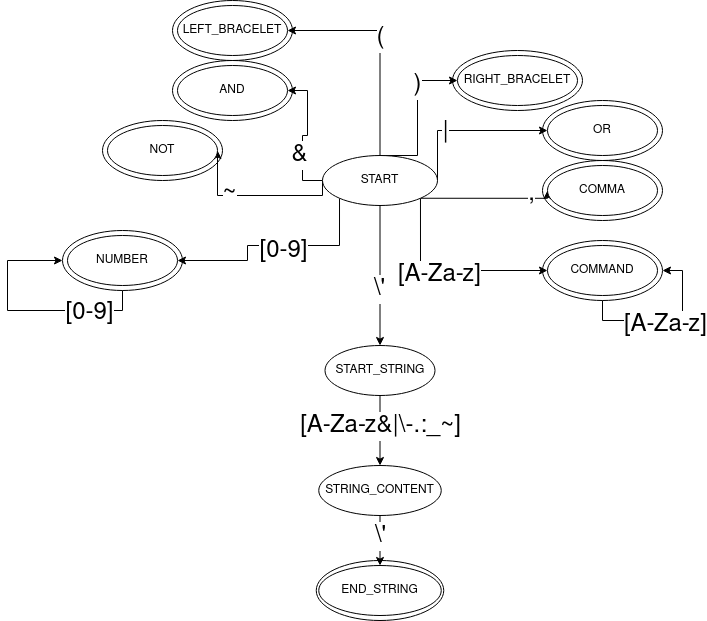
\includegraphics[scale=0.5]{obrazky-figures/RPQR_FSM.png}

\newpage

The lexical tokens that occure in RPQR language are:
\begin{itemize}
  \item left bracelet (
  \item right bracelet )
  \item and operator \&
  \item or operator |
  \item negation operator ~
  \item number (consisting only of numeric characters e.g 123)
  \item string (hyphen separated string of alphanumeric and special characters e.g 'hello')
  \item command (command contains only alpha characters and has to be described by a plugin e.g NAMELIKE)
  \item comma used mainly as a separator for command arguments ,
\end{itemize}

\subsection*{Syntactic analysis}
RPQR language syntactic analysis will be mainly precedent syntactic analysis because the language is statement
oriented. Precedent syntactic analysis uses algorithm with symbol stack and acts accordingly to precedent
syntactic table. This table defines what operators can be used at particular places and their respective
priorities. This solves the problem of evaluation of statement but there is still the matter of command
recognition and validation of argument types. Every command has to define what arguments it needs to work
properly. Initial configuration of RPQR will load commands and create context less gramatic for them.
Because every command has different name and there is no need for dynamic arguments, distinction should
be straightforward and effective.

Another more problematic matter is that for RPQR language to be able to handle all neccessary use cases,
commands need to be able to accept results of other commands as arguments. This is problematic, since
it requires new instance of precedent syntactic analysis to parse this statement. Fortunately this
can be solved by cutting substatement out of original statement and putting it queue of statements
that have to be yet parsed.

After all these problems are solved, RPQR will have abstract syntactic tree containing all the information
that is neccessary for exectution of statement e.g. commands that need to be executed first and operators
located in depth accordingly to their precendence. This tree will be later processed by semantic
analysis e.g. interpreter.

\newpage

Precedent syntactic table used for RPQR language:

\begin{center}
  \begin{tabular}{ |c|c|c|c|c|c|c| }
   \hline
     & ( & ) & \& & | & \textasciitilde & \$ \\
     \hline
  (  & < & = & <  & <  & <  & \#  \\
  \hline
  )  & \# & > & >  & >  & >  & >  \\  
  \hline
  \& & < & > & >  & <  & <  & >  \\
  \hline
  |  & < & > & <  & >  & <  & >  \\
  \hline
  \textasciitilde  & < & > & >  & >  & <  & >  \\
  \hline
  \$ & < & \# & <  & <  & <  & X \\
  \hline
  \end{tabular}
\end{center}

\textbf{Explanation of symbols}

Algorithm which handles syntactic analysis is driven by the precedent syntactic table. It always
looks at the first terminal symbol at the top of the stack and performs operation that is specified
in table by what symbol is in input.
\begin{itemize}
  \item < means that special symbol marking start of particular statement needs to be put onto stack and new symbol loaded from input
  \item = means only load new symbol
  \item > means that particular sub statements should be collapsed into one parent statement
  \item \# means that syntactic error occured and provided input is not a valid RQPR language statement
\end{itemize}

\subsection*{Semantic analysis}
Semantic analysis e.g. interpreter will be implementation of depth first search algorithm for processing
of abstract syntactic tree provided by syntactic analysis. It is walking through the tree and putting
found nodes in a stack until it finds command or statement that can be already resolved. When command
that is defined by accessible plugin is encountered, then interpreter will filter loaded packages and
either provide them as final result or use them as an operand to one of the operators.

When command is executed or statement can be evaluated accordingly to type of operator that it
contains, part of abstract syntactic tree related to it is marked as resolved and temporary result
is saved into the appropriate node. This means that the final result will be present as a root
of the tree.

As in syntactic analysis, there is a problem with subsets used as an arguments. These subsets have
to be executed in simmilar manner as they were processed into abstract syntactic tree. When encountered
interpreter will stop command processing and proceed to resolving the substatement with higher priority.

\section{RPQR language and its use}
This section should provide usage examples of RPQR language and results that should be expected.
RPQR statement always consists of at least one command.

\subsection*{Simple command}

\textit{COMMAND()}

This command will receive the entire graph of packages as input and will be responsible for providing
set of packages that conform to its filter. Since this command does not accept any arguments, as there
are no arguments supplied, the filter is static and can not be affected by user.

\subsection*{Command with arguments}

\textit{ADVANCEDCOMMAND('package', 3)}

Command used like this accepts two arguments which alter his behaviour. The first one is a string
and the second is a number. RPQR language does not consider whitespace characters, so there is no
difference or problem with their presence in query. Commands like this can have more advanced
behaviour and are generally more useful.

\subsection*{Command accepting subset as an argument}

\textit{SUBSETCOMMAND(NAMELIKE('cups'), 3)}

This is the most complex command that RPQR language supports. This query will at first filter the
entire graph with command \textit{NAMELIKE('cups')} and then supply its result to the \textit{SUBSETCOMMAND}
command. The second command will have possibility to work with subset and thus does not have to
work with the entire graph which results in ability to work more efficiently or perform operations
with specific context. For better explanation how the query could work. The first command could
gather packages which contain string \textit{cups} in their name. The second could then filter only
three first by their name in alphabetical order.

\newpage

\subsection*{Operators}

\textbf{Intersection}

\textit{FIRSTCOMMAND() \& SECONDCOMMAND()}

Operator \& can be used as a intersection between sets provided as outputs of two commands or sets.
Packages returned by query specified like this have to be present in both left and right set.

\textbf{Join}

\textit{FIRSTCOMMAND() | SECONDCOMMAND()}

Operator | can be used to join sets provided by two commands or statements. It has lower priority
than intersection and means that resulting sets will contain packages that are present in either
left or right set of this statement.

\textbf{Negation}

\textit{\textasciitilde FIRSTCOMMAND()}

Operator \textasciitilde can be used to specify that result set of packages can contain only such
packages that does not conform to conditions specified by \textit{FIRSTCOMMAND}. It is important
to keep in mind that input of the command is always the entire graph.

\subsection*{Complex queries and explanation of their semantics}

When in need of complex conditions and combination of commands, it is very useful to use bracelets
to force priority of evaluation and to avoid confusion between what user expects as a result and
what is the real result.

\textbf{Example of bracelet use:}

\textit{FIRSTCOMMAND() \& SECONDCOMMAND() | THIRDCOMMAND()}

Explanation of this query is: return packages that conform to conditions of \textit{FIRSTCOMMAND}
and \textit{SECONDCOMMAND} or packages that conform to \textit{THIRDCOMMAND}. This is caused
by priority of operators.

\textit{FIRSTCOMMAND() \& (SECONDCOMMAND() | THIRDCOMMAND())}

This query looks very simmilar but there are bracelets that change its meaning very significantly.
Packages in result set has to conform to \textit{FIRSTCOMMAND} and to \textit{SECONDCOMMAND} or 
\textit{THIRDCOMMAND} in the same time. Bracelets allow us to form more complex descriptions of
packages that we are looking for.

\section{Plugin architecture and its interface}

Since the whole project will be written in Python which is object oriented language, all plugins
will be inheriting from class that will provide standard interface expected by RPQR project. There
should be initialization method allowing plugin to prepare helper structures and then method responsible
for inserting information into the plugins. Packages have attributes and relationships, so there 
will have to be two type of plugins, one inserting proper attributes to nodes and another one that
will construct relationships between them. RPQR will work with attribute plugins as if they had
a higher priority so relationship plugins will be able to work with already prepared attributes and
there will be no unnecessary overhead.

Commands supplied by plugin will also conform to interface specified by their base class. Each
will have to list types of arguments that they need and implement function that contains logic of
their filtering operations. Since many commands will be working with simmilar graph algorithms such as
depth first search or breadth first search, base class will provide optimalized implementation that
just needs specification of filter in a form of function.

\section{Caching}

As was stated in previous chapter, RPQR will need to use cache to save time consumed by building information
about packages contained in configured repositories. After careful consideration, the approach with
using JSON as a format of cache was choosen. This way, even third party tools will be able to manipulate
with it and users will be able to read it if neccessary. Cache will be invalidated only by users
request to do so and when new plugin is found. Presence of plugins will be tested by special record
in cache. Fortunately all this is supported by networkX library.

\section{API design}
RPQR needs to have Python application programming interface so external developers can use its plugins
and features even more efficiently than through command line interface and create their own solutions.
API will be using the same RPQR language as command line interface and queries will be returning
networkx graphs. This way, applications using the API can walk through nodes that represent packages
and perform any transformation of graph that they deem useful.

\newpage

\section{Command line interface design}
RPQR tool will be using one main positional option that has to be provided and that is a query written
in RPQR language. By default the output will go into standart output and log messages to standard error output.

First two options that can, but does not have to be specified will be whether user wants to see visualization
of result created by his query and what attributes or relations should be included in the output.
Filtering of attributes and relations is helpful because with multiple plugins, there can be a lot
of unnecessary data in the output that take a lot of space. Another important option is location
of configuration file if user does not want to use the default location which is \textit{/etc/rpqr.conf}.
The last option is whether the tool should invalidate cache and build it again.

\chapter{Implementation and evaluation}
With research and design complete, RPQR project can now be implemented in a best way possible.
This chapter will cover deep description of projects code and algorithms it uses to fulfill the
assigned task. Each section will cover limitations of presented solution and what could be done
in the future to overcome them. Usage of RPQR project will also be described in a form of user
manual and description of a way how new plugins are supposed to be developed using RPQR interface.

\section{Important parts of implementation}
This section will show the most important parts of implemenation and structure of Python code.

\subsection*{RPQRConfiguration}
RPQRConfiguration class serves for purposes of loading plugins and creating RPQR language structures
neccessary for its successful parsing and interpreting. Instance of this class has to be created for
every use of RPQR project and is used by all following components and their diverse operations.

\newpage

\textbf{Initialization of plugins}

\begin{lstlisting}
def _initializePlugins(self):
  """ Load plugins from supplied directories
  """
  for dir in self.pluginDirectories:
      sys.path.append(dir)
      pluginModules = os.listdir(dir)
      for file in pluginModules:
          moduleName = file[:-3]
          # if file name starts with _ then it is most likely not a plugin
          if moduleName.startswith("_"):
              continue
          cfg = None
          if moduleName in self.userConfiguration.keys():
              cfg = self.userConfiguration[moduleName]

          if (cfg != None and cfg.get("disabled") == "1"):
              self._logger.info(
                  "%s plugin was disabled in configuration" % moduleName)
              continue
          module = importlib.import_module(moduleName)
          pluginClass = getattr(module, moduleName)

          pluginInstance = pluginClass(rootLogger=self.rootLogger,
                                      config=cfg)
          self.plugins.append(pluginInstance)
\end{lstlisting}

This is the centerpiece of plugin loading. This method walks through all configured directories
which according to configuration should contain plugin modules and if its file does not start with
an underscore then attempts to import them and create their instance. There are two conditionals
which relate to plugin configuration. The first one is checking whether a configuration related to
this plugin exists and thus should be provided to it and the second one is there for a case when
user does not want to use plugin at all, to save space for example or to speed up processing.

\subsection*{RPQRLoader}
RPQRLoader is a class responsible for loading of data about packages through plugins and constructing
graph structure out of them. It is taking advantage of DNF API to retrieve the data as efficiently as
possible and access them in the same way as package manager would.

\newpage

\textbf{Construction of graph}

\begin{lstlisting}
def createDatabase(self, cache: str = None) -> networkx.MultiDiGraph:
  """ Get graph of packages with data and relations described by plugins

  :param cache: path to cache file, defaults to None
  :type cache: str, optional
  :return: Graph of packages
  :rtype: networkx.MultiDiGraph
  """
  graph = networkx.MultiDiGraph()
  dataPlugins = [plugin for plugin in self.plugins if isinstance(
      plugin, RPQRDataPlugin)]
  relationPlugins = [plugin for plugin in self.plugins if isinstance(
      plugin, RPQRRelationPlugin)]

  pluginRecords = []
  for plugin in dataPlugins + relationPlugins:
      pluginRecords.append((plugin, plugin.__class__.__name__))

  ...

  av_query = self._getAvailableQuery()
  q_avail = av_query.run()

  for id, pkg in enumerate(q_avail):
      graph.add_node(id)
      for pluginInstance in dataPlugins:
          pluginInstance: RPQRDataPlugin
          pluginInstance.fillData(id, pkg, graph)

  for id, pkg in enumerate(q_avail):
      for pluginInstance in relationPlugins:
          pluginInstance: RPQRRelationPlugin
          pluginInstance.fillData(id, pkg, graph, av_query)

  graph.graph["plugins"] = [name for (_, name) in pluginRecords]
  ...
  return graph
\end{lstlisting}

This method distinguishes between plugins that are supposed to add attributes to package nodes and
plugins that create relations between individual packages. The first kind is executed first so
relationship plugins can depend on them later. Each instance of plugin has its fillData method
which is called for each package that was retrieved by DNF API. After the graph is build, list
of plugins that were present during creating of this structure is saved into plugins list for easier
detection of invalid cache.

\subsection*{RPQRScanner}
RPQRScanner is a class responsible for scanning of query entered in RPQR language format. It is able
to recognize when there is a lexical error in the query and is used to parse string into tokens.

\textbf{Implementation of finite state machine}

\begin{lstlisting}
def getTokens(self, input: str) -> Optional[List[RPQRToken]]:
  ...
  while curInputIndex < len(input) + 1:
      if curInputIndex < len(input):
          c = input[curInputIndex]
      else:
          c = ''
      if curState == States.START:
          if c == '':
              break
          elif c == '(':
              curToken = RPQRToken(self.tokenTypes["leftBracelet"], c)
              curState = States.LEFTBRACELET
          elif c == ')':
              curToken = RPQRToken(self.tokenTypes["rightBracelet"], c)
              curState = States.RIGHTBRACELET
          elif c == '&':
              curToken = RPQRToken(self.tokenTypes["and"], c)
              curState = States.AND
          ...
          curInputIndex += 1
      elif curState == States.AND:
          tokens.append(curToken)
          curState = States.START
      elif curState == States.OR:
          tokens.append(curToken)
          curState = States.START
      elif curState == States.NUMBER:
          if c.isnumeric():
              curToken.appendToContent(c)
              curInputIndex += 1
          else:
              tokens.append(curToken)
              curState = States.START
\end{lstlisting}

Method getTokens is responsible for creating a list of tokens out of input. It is composed out of
while cycle which parses characters and switches state of the machine accordingly. It is strictly
implemented accordingly to graph of FSM which was mentioned earlier.

\subsection*{RPQRParser}

RPQRParser is a class responsible for processing of lexical tokens and construction of abstract syntactic
tree that can be interpreted in a strictly defined way. The class contains helper methods for easier
manipulation with list of tokens and methods considered as callbacks to certain operations encountered
in source query. These operations are uses of operators like \textit{\&} or \textit{\textasciitilde}
which need the abstract syntactic tree to be constructed in a certain way.

\textbf{parsing algorithm}

\begin{lstlisting}
while True:
  while True:
      if curInput.type in self.config.commandTypes.values():
          commandRule = None
          for rule in self.rules[4:]:
              if rule[0] == curInput.type:
                  commandRule = rule
          childList = [curInput]
          for indexMember, member in enumerate(commandRule[1:]):
              # if command requires substatement, then cut its tokens
              # and put it into queue
              if member == self.nonTerminalTypes["statement"]:
                ...
              if argToken.type != member:
                ...
              if argToken.type in [self.config.tokenTypes["number"], self.config.tokenTypes["string"]]:
                  childList.append(argToken)
          newStatement = RPQRStackSymbol(
              self.nonTerminalTypes["statement"], childList)
          self.stack.append(newStatement)
          curInput = tokens.pop(0)
          continue

      lastTerminalIndex = 0
      ...

      requiredAction = precedencTable[self.stack[lastTerminalIndex].type][curInput.type]
      ...
  # decide whether we need to keep parsing or everything is already done
  if len(substatementQueue) == 0:
      return rootStatement
  else:
      curStatement = substatementQueue.pop(0)
      self.stack = [RPQRStackSymbol(self.config.tokenTypes["end"])]
      tokens = curStatement.children
      curInput = tokens.pop(0)
\end{lstlisting}

Parsing algorith is based on processing of statement queue that contains all individual statements
that need to be parsed. The first cycle is going through queue of statements and the inner one is
performing precedent syntactic analysis and calling appropriate callbacks. Interesting operation is
that when substatement is encountered (command accepts statement as an argument) algorithm cuts this
substatement out of the source and inserts it into the queue for further resolution. Because of trees
structure, it is possible to resolve rest of the statement even when construction of substatement is not yet
known.

Current parsing algorithm is not able to handle commands that take dynamic number of arguments. This
is a known limitation but because this feature was not needed in any relevant testing scenario,
RPQR will not in time of this thesis contain such option.

\newpage

\subsection*{RPQRInterpreter}

RPQRInterpreter is a class responsible for interpretation of RPQR language. It is mainly composed out
of a algorithm which performs depth first search of abstract syntactic tree and resolves nodes from
bottom to up direction.

\textbf{Interpretation algorithm}

\begin{lstlisting}
while len(stack) > 0:
    curNode = stack[-1]
    curResult = resultStack[-1]
    if curNode.operator is not None:
        if len(curResult.childResults) < 1:
            ...
        elif curNode.operator != '~' and len(curResult.childResults) < 2:
            ...
        else:
            # now we have all operands, we can begin resolution
            validNodes = []
            ...
            stack.pop()
            resultStack.pop()
    else:
        ...
        notResolvedStatementFound = False
        for argIndex, argType in enumerate(commandClass.args):
            if argType == str or argType == int:
                # literals can be resolved right away
                if (argIndex > len(curResult.childResults)-1):
                    curResult.childResults.append(RPQRResultTree(
                        curNode.children[1:][argIndex].content, []))
                else:
                    continue
            elif argType == list:
                if (argIndex > len(curResult.childResults)-1):
                    ...
                    break
                else:
                    continue
        if notResolvedStatementFound:
            continue
        arguments = []
        for partResult in curResult.childResults:
            arguments.append(partResult.result)
        curResult.result = commandClass.execute(graph, arguments)
        stack.pop()
        resultStack.pop()
\end{lstlisting}

Algorithm distinguishes between nodes that represent statement composed out of operator and operands
and commands that filter packages. Processing of such nodes differs, because operators are built in
and have fixed number of arguments while commands are defined by plugins and every command can have
different number of arguments. Algorithm walks through abstract syntactic tree and performs partial
operations by calling execute method of plugins with already loaded arguments. When the root node
is reached by resolution and its result is known, then the result can be returned by \textit{performCommands}
method and formated by users requirements.

\newpage

\subsection*{RPQR script}
RPQR script is a command line utility which allows user to use RPQR project comfortably. It is designed
to take advantage of the whole project and its features while providing user with the ability to
controll for example when a cache file should be invalidated and overwritten.

\textbf{RPQR script implemenation}

\begin{lstlisting}
  rpqrcfg = RPQRConfiguration(pluginDirectories, namexrepository, cfgParser)
  loader = RPQRLoader(rpqrcfg)

  graph = loader.createDatabase(cacheFile, args.clearcache)
  # we will not be performing empty query
  if len(args.query) == 0:
      sys.exit(0)
  result = RPQRQuery.performQuery(args.query, graph, rpqrcfg)

  if result is None:
      sys.exit(1)

  # we will filter result attributes according to supplied parameters
  if len(args.filterattributes) != 0 or len(args.filterrelations) != 0:
      ...
      if len(args.filterattributes.split(";")[0]) != 0:
          for node in result.nodes:
              for key in list(result.nodes[node].keys()):
                  if not key in args.filterattributes.split(";"):
                      del result.nodes[node][key]
      if len(args.filterrelations.split(";")[0]) != 0:
          for node in result.nodes:
              for u, v, edge_key in graph.out_edges([node], keys=True):
                  if not edge_key in args.filterrelations.split(";"):
                      graph.remove_edge(u, v, key=edge_key)

  # if result should not be visualized then just print it in JSON format to stdout
  if not args.visualize:
      print(json.dumps(json_graph.node_link_data(
          result), indent=4, sort_keys=True))
      sys.exit(0)

  # labeling requires some more processing
  ...
  pos = networkx.spring_layout(result)
  networkx.draw_networkx(result, pos=pos, with_labels=True, labels=labelDict)
  edgeLabels = dict([((n1, n2), key) for n1, n2, key in result.edges])
  networkx.draw_networkx_edge_labels(result, pos=pos, edge_labels=edgeLabels)
  plt.show()
\end{lstlisting}

Implementation of RPQR script uses RPQR API and allows user to specify whether the result should be
visualized or printed out through the standard output. Another very useful feature is filtering of
attributes and relations that should be included in the output. Script is using matplotlib python
library to render graph of packages if required.

\section{User manual}
This section contains manual of RPQR tool and detailed description of a way how it is intended to be
used. Another part provides information about developing of plugins and scripts that are using RPQR
API to retrieve and filter package metadata.

\textbf{NAME}

RPQR - RPM package query resolver

\textbf{SYNOPSIS}

RPQR [-h] [--cfgpath CFGPATH] [--filterattributes FILTERATTRIBUTES] [--filterrelations FILTERRELATIONS]
[--visualize] [--clearcache]
query

\textbf{DESCRIPTION}

RPQR utility is supposed to make querying RPM repositories about package metadata easy by providing
user with means to filter them by such metadata and individual types of relations that occure between
them. Utility is configurable through configuration file which is located by default in \textit{/etc/rpqr.conf}.

\textbf{OPTIONS}

\begin{itemize}
  \item -h, --help
    \subitem Show help message and exit
  \item --cfgpath CFGPATH
    \subitem Path to configuration file
  \item --filterattributes FILTERATTRIBUTES
    \subitem Specify list of attributes which interest you in the result. If left empty, then all attributes will be present in result
  \item --filterrelations FILTERRELATIONS
    \subitem Specify list of relations which interest you in the result. If left empty, then all relations will be present in result
  \item --visualize
    \subitem Visualize result
  \item --clearcache
    \subitem Clear cache
\end{itemize}

\textbf{CONFIGURATION FILE}

Following configuration file should illustrate general principles of how the RPQR utility behaviour
can be changed with it.

\begin{lstlisting}
[RPQR]
pluginDirectories=["./rpqr/loader/plugins/implementations"]
cache=/var/tmp/rpqr.json

[RPQRRepo_f34-repo]
url=http://ftp.fi.muni.cz/pub/linux/fedora/linux/releases/34/Everything/x86_64/os/

[RPQRMaintainerPlugin]
url=https://src.fedoraproject.org/extras/pagure_owner_alias.json
\end{lstlisting}

First section named \textit{RPQR} is main configuration section that contains the most important
setting. \textit{pluginDirectories} is array of directories which contain python modules with RPQR
plugins. \textit{cache} is path to cache file, when this path is not supplied then RPQR utility
will not use cache.

Second section named \textit{RPQRRepo\_f34-repo} is meant to set up repository which user wants to
query. There can be one to n number of repositories and they all have to be configured in their own
section with prefix \textit{RPQRRepo\_} and member url which specifies base URL of the repository.

The third section is required for \textit{RPQRMaintainerPlugin}. Each plugin can have its own section
of configuration and member disabled, which when set to \textit{1} will prevent this plugin from
working. Plugin configuration is described by plugins individually and is mentioned here only for
clarification of example.

\textbf{Example of use}

RPQR "ONWHATDEPENDS('libyang-1.0.225-1.fc34.x86\_64', 1)" --filterattributes "name" --filterrelations "depends" --visualize

\textbf{RPQR language}

RPQR language serves as a means to specify what packages user wants to see in result. Take advantage
of operators to create appropriate combination of commands to get the results that you want.

\textbf{Operators}

\begin{itemize}
  \item \& - package has to conform to both right and left statements
  \item  | - package has to conform to either left or right statements
  \item  \textasciitilde - package must not conform to statement located on the right 
\end{itemize}

\newpage

\textbf{Parenthesis}

RPQR also supports parenthesis to provide further means to set priority of statements that are specified.
Use parenthesis to make your query more readable and to make sure that the result is what you expect.
\textit{statement1 \& (statement2 | statement3)} This statement is not equal to the version without
parenthesis specified like this \textit{statement1 \& statement2 | statement3}. Semantic of the first
statement is: \textbf{Find packages that conform to statement1 and in the same time conform to either
statement2 or statement3}. On the other hand, the second statement meaning is: \textbf{Find packages
that conform to both statement1 and statement2 but if package conforms to statement3 then it does not
have to conform either to statement1 or statement2}

\textbf{Official distributed plugins documentation}

This section of the manual contains documentation about behaviour of plugins that are officially
distributed with the RPQR tool and supported by the maintainers.

\textbf{RPQRNamePlugin}

RPQRNamePlugin is one of the most important plugins for RPQR utility. It gathers complete name of the
package, meaning its name, version, release and architecture. It is an attribute plugin and inserts
attribute \textit{name} into the package.

\begin{itemize}
  \item Added attribute: 'name'
  \item Added commands: 'NAME', 'NAMELIKE', 'SUBSETNAMELIKE'
  \item Depends on plugins: None
\end{itemize}

\textbf{Commands provided by RPQRNamePlugin}

\textbf{NAME}

Required arguments: name (string literal)

\textit{NAME} command filters out only package that has the exact same name attribute as was specified
with the name argument.

Example of use: \textit{NAME('libyang-1.0.225-1.fc34.x86\_64')}

\textbf{NAMELIKE}

Required arguments: name (string literal)

\textit{NAMELIKE} command filters out packages that contain substring specified with the argument
\textit{name}.

Example of use: \textit{NAMELIKE('libyang')}

\newpage

\textbf{SUBSETNAMELIKE}

Required arguments: name (string literal), statement (RPQRLanguage statement)

\textit{SUBSETNAMELIKE} command filters out packages returned by argument \textit{statement} that
contain substring specified with the argument \textit{name}.

Example of use: \textit{SUBSETNAMELIKE('x86\_64', NAMELIKE('libyang'))}

Explanation of the example semantics: This query returns packages that contain \textit{libyang} in their
name and in the same time \textit{x86\_64} substring. Difference between this statement and
\textit{NAMELIKE('x86\_64') \& NAMELIKE('libyang')} is that the first query will be faster, because
it has to go through only subset of packages.

\textbf{RPQRDependencyPlugin}

RPQRDependencyPlugin is relation plugin which gathers information about package dependencies and
creates dependency relations between nodes that represent them in RPQR graph of packages.

\begin{itemize}
  \item Added relation: 'depends'
  \item Added commands: 'ONWHATDEPENDS', 'WHATDEPENDSON'
  \item Depends on plugins: RPQRNamePlugin
\end{itemize}

\textbf{Commands provided by RPQRDependencyPlugin}

\textbf{ONWHATDEPENDS}

Required arguments: name (string literal), depth (numeric literal)

\textit{ONWHATDEPENDS} command filters out packages on which package, with name attribute matching
\textit{name} argument, depends. \textit{depth} argument is controlling the depth to which RPQR
should go when gathering dependencies from the graph. Depth zero means that only the package specified
by name will be present in output, value one causes that only direct dependencies will be present and
so on.

Example of use: \textit{ONWHATDEPENDS('libyang-1.0.225-1.fc34.x86\_64', 1)}

\textbf{WHATDEPENDSON}

Required arguments: name (string literal), depth (numeric literal)

\textit{WHATDEPENDSON} command filters out packages that depend on package, with name attribute matching
\textit{name} argument. \textit{depth} argument is controlling the depth to which RPQR
should go when gathering dependent packages from the graph. Depth zero means that only the package specified
by name will be present in output, value one causes that only directly dependendent packages will be present and
so on.

Example of use: \textit{WHATDEPENDSON('libyang-1.0.225-1.fc34.x86\_64', 1)}

\textbf{RPQRMaintainerPlugin}

RPQRMaintainerPlugin is an attribute plugin which gathers information about maintainers which work
on packages. It inserts attribute \textit{maintainer} into packages. Plugin unfortunately depends
on the format of list of maintainers which has to be in JSON.

\begin{itemize}
  \item Added attribute: 'maintainer'
  \item Added commands: 'MAINTAINER', 'DEPENDSONUSER'
  \item Depends on plugins: RPQRDependencyPlugin
\end{itemize}

\textbf{Commands provided by RPQRMaintainerPlugin}

\textbf{MAINTAINER}

Required arguments: maintainers name (string literal)

\textit{MAINTAINER} command filters out packages that have maintainer specified with argument
maintainers name in list of their maintainers.

Example of use: \textit{MAINTAINER('tkorbar')}

\textbf{DEPENDSONUSER}

Required arguments: maintainers name (string literal), depth (numeric literal)

\textit{DEPENDSONUSER} command filters out packages that depend on work of maintainer specified with
argument \textit{maintainers name}. That means that depth zero will retrieve packages that have specified
maintainer in list of its maintainers as \textit{MAINTAINER} command would. Values higher than zero
will retrieve packages that depend on those retrieved with depth zero.

Example of use: \textit{DEPENDSONUSER('tkorbar', 1)}

\textbf{RPQRMaintainerPlugin configuration}

RPQRMaintainerPlugin has one additional variable for configuration not included in the default set for
all plugins. It is variable url which specifies location of maintainer list.

Example:
\begin{lstlisting}
[RPQRMaintainerPlugin]
url=https://src.fedoraproject.org/extras/pagure_owner_alias.json
\end{lstlisting}

\textbf{LICENSE}

You may copy, distribute and modify the software as long as you track changes/dates in source files.
Any modifications to or software including (via compiler) GPL-licensed code must also be made available
under the GPL along with build \& install instructions.

\section{API documentation and example of scripting}

RPQR project allows developers to create their own plugins which can further extend its ability to
recognize attributes and relations between packages. This section will show already existing plugins
on which it will describe plugin development and importance of individual parts.

\subsection*{RPQRMaintainerPlugin}

\begin{lstlisting}
  class RPQRMaintainerPlugin(RPQRDataPlugin):
    """ Plugin allowing us to store information about package maintainers
        and ask Queries about them
    """
\end{lstlisting}

Plugin which wants to add new attribute to packages needs to inherit from RPQRDataPlugin class.
Please pay attention to file name of your python module. The file name has to be the same as
name of the class.

\begin{lstlisting}
    desiredName = "maintainer"

    implementedCommands = [MaintainerFilter, DependsOnUserFilter]
\end{lstlisting}

\textit{desiredName} is a name of the attribute that this plugin wants to add. \textit{implementedCommands}
is a list of classes of commands that this plugin wants to add to RPQR project. Commands will be described
later.

\begin{lstlisting}
    packageToMaintainer = None

    def __init__(self, rootLogger: Logger = None, config: dict = None):
        self.listUrl = None
        if config == None and rootLogger != None:
            lgr = rootLogger.getChild("RPQRDataPlugin")
            lgr.warning("url for retrieval of maintainers was not supplied")
            return

        self.logger = rootLogger.getChild(
            "RPQRDataPlugin") if rootLogger != None else None

        self.listUrl = config.get("url")
\end{lstlisting}

\textit{packageToMaintainer} is a helper class variable. Plugin can declare its variables as it sees
fit. Plugin needs to be ready for usecases when it does not has access to logger or configuration
and has to act accordingly. Because \textit{RPQRMaintainerPlugin} needs to know url for retrieval
of maintainer list, it has to access configuration. All such usecases have to be documented.

\newpage

\begin{lstlisting}
    def _downloadJson(self):
        if self.listUrl == None:
            return {}
        receivedResponse = requests.get(self.listUrl)

        if receivedResponse.status_code != 200:
            self.logger.error(
                "RPQR was unable to retrieve maintainer list from supplied url %s" % self.listUrl)

        return receivedResponse.json().get("rpms", {})
\end{lstlisting}

This is a helper method for retrieval of maintainer list. Plugins can access any source of information
that they want but this also has to be documented.

\begin{lstlisting}
    def prepareData(self, pkg: hawkey.Package) -> List[str]:
        """Get maintainers of package

        :param pkg: hawkey package information
        :type pkg: hawkey.Package
        :return: list of maintainers
        :rtype: List[str]
        """
        # download package maintainer list and build dictionary from it
        if RPQRMaintainerPlugin.packageToMaintainer is None:
            RPQRMaintainerPlugin.packageToMaintainer = {}
            data = self._downloadJson()
            data: dict
            for name, value in data.items():
                RPQRMaintainerPlugin.packageToMaintainer[name] = value
        # owner alias json uses source names as keys
        return RPQRMaintainerPlugin.packageToMaintainer[pkg.name if pkg.source_name == None else pkg.source_name]
\end{lstlisting}

\textit{prepareData} is called for each individual package and has to return value which should be
saved to the implemented attribute. If block is there, because first run of this method will retrieve
list of maintainers and create helper dictionary to accelerate loading. Please use such approaches
to keep the project fast. After such initialization, for every package is just returned list of maintainers
from \textit{packageToMaintainer} dictionary. The ternary operator is there, because source packages
have different naming conventions in dnf API than the binary ones and RPQR has to be ready for both.

\newpage

\subsection*{DependsOnUserFilter}

\begin{lstlisting}
  class DependsOnUserFilter(RPQRFilteringCommand):
    """Command allowing filtering packages which depend on certain maintainer.
    That means the person is either maintaining them or package depends on
    package which they maintain recursively.
    """
    args = [str, int]
    name = "DEPENDSONUSER"

    def execute(graph: networkx.MultiDiGraph, args: list) -> List[int]:
        """ Get list of ids of packages which depend on user specified in args[0]
        to max depth args[1]

        :param graph: built graph of packages
        :type graph: MultiDiGraph
        :param args: arguments supplied to command
        :type args: list
        :return: node ids of packages which depend on specified maintainer
        :rtype: List[int]
        """
        targetUser = args[0]
        depth = int(args[1])
        nodes = [a for a in list(graph.nodes)
                 if targetUser in graph.nodes[a]["maintainer"]]

        return RPQRFilteringCommand._BFS(graph, nodes, depth, "depends")
\end{lstlisting}

This is more complex command out of \textit{RPQRMaintainerPlugin}s two commands so it is more worthy of
explanation. All commands have to inherit from \textit{RPQRFilteringCommand} class and declare \textit{args}
array and \textit{name} class variable. \textit{args} is a array which tells RPQR project what arguments
this command needs. Allowed types are str, int and list. Str means string literal, int means numeric
literal and list is a result of substatement. List is handled as list on integers. \textit{name}
is name of the command used to invocate it.

All commands have to implement \textit{execute} method. \textit{execute} method receives built graph
of packages and its arguments. As you can see, first command gathers ids of nodes which have specified
maintainer in their maintainer list. Ids are then passed to static method \_BFS which is prepared
implementation of Breadth First Search. Breadth First Search then finds dependent nodes to specified
depth.

\newpage

\subsection*{RPQRDependencyPlugin}

\begin{lstlisting}
  class RPQRDependencyPlugin(RPQRRelationPlugin):
    """Plugin for gathering dependencies of packages and allowing filtering
    by them
    """
    desiredName = "depends"
    implementedCommands = [OnWhatDependsFilter, WhatDepensOnFilter]

    def __init__(self, rootLogger: Logger = None, config: dict = None) -> None:
        self.optionalDataStructure = None

    def prepareData(self, pkg: hawkey.Package, graph: MultiDiGraph, query: hawkey.Query) -> List[int]:
        """ Get list of nodes to which we want to form this relation

        :param pkg: hawkey package object. Holds information supplied by dnf api
        :type pkg: hawkey.Package
        :param graph: graph of packages
        :type graph: MultiDiGraph
        :param query: hawkey query object. Allows further queries through dnf api
        :type query: hawkey.Query
        :return: list of target nodes for this node
        :rtype: List[int]
        """
        # we will use dictionary for optimalization of this process
        if self.optionalDataStructure == None:
            self.optionalDataStructure = {}
            for (node, attribs) in graph.nodes.items():
                self.optionalDataStructure[attribs["name"]] = node

        edges = list()
        requiredPackages = query.filter(provides=pkg.requires).run()
        for dependency in requiredPackages:
            target = self.optionalDataStructure[str(dependency)]
            edges.append(target)
        return edges
\end{lstlisting}

Relation plugins are very simmilar to those adding attributes with a few differences. Relation plugins
are able to access graph of packages which they can access and hawkey query from DNF API. Relation
plugins are returning list of target nodes of oriented edges that they are creating.

\section{Use of RPQR API to perform queries}

Working of RPQR API will be described on the \textit{RPQROrphaned} script which was used for testing
of RPQR project.

\begin{lstlisting}
  if __name__ == "__main__":
    # set up configuration
    config = RPQRConfiguration([os.path.dirname(rpqr.loader.plugins.implementations.__file__)],
                               [("fedora-repo", "http://ftp.fi.muni.cz/pub/linux/fedora/linux/releases/33/Everything/x86_64/os/"),
                                ("source-repo", "http://ftp.fi.muni.cz/pub/linux/fedora/linux/releases/33/Everything/source/tree/")],
                                {"RPQRMaintainerPlugin":{"url": "https://src.fedoraproject.org/extras/pagure_owner_alias.json"}})
    query = RPQRQuery(config)
    result = query.performQuery("MAINTAINER('orphan')")
    for node in list(result.nodes):
        # now we will recursively gather packages which depend on every orphaned package
        dependentPackages = query.performQuery(
            "WHATDEPENDSON('%s', 20)" % result.nodes[node]["name"])
        # get maintainers affected by this change
        maintainerList = []
        for pkgId in list(dependentPackages.nodes):
            for maintainer in dependentPackages.nodes[pkgId]["maintainer"]:
                if maintainer not in maintainerList:
                    maintainerList.append(maintainer)
        maintainerList = list(dict.fromkeys(maintainerList))
        # orphan is just a placeholder so remove it
        maintainerList.remove('orphan')
        print("%s => " % dependentPackages.nodes[node]["name"], end="")
        for maintainer in maintainerList:
            print("%s " % maintainer, end="")
        print()
\end{lstlisting}

Every use of the API needs to start with creating of an instance of \textit{RPQRConfiguration} class.
After that, the only other required thing is instance of \textit{RPQRQuery} class and then it is
possible to create perform queries. Results are returned as a \textit{networkx} graph and has to be
worked with as. This script walks through orphaned packages and finds other maintainers affected by
their orphanation. 

\chapter{Conclusion}

\blindtext